\chapter{موسیقی}
\section{مدیاپایپ}
برای این پروژه ما از مدل از قبل آموزش داده شده\LTRfootnote{Pretrained} در کلاس مدیاپایپ که مخصوص نقاط عطف دست است استفاده میکنیم. مدیاپایپ  از یک خط لوله
یادگیری ماشین متشکل از چندین مدل که با هم کار می کنند استفاده می کند: یک مدل تشخیص کف دست \LTRfootnote{Palm detection model}
که تصویر را از ورودی می‌گیرد و  عکس محدوده دست را به عنوان خروجی دریافت میکند و یک مدل تشخیص نقاط عطف دست \LTRfootnote{Hand landmark model}
که عکس دست را به عنوان ورودی گرفته و مختصات‌ 21 نقطه کلیدی بند‌های انگشتان دست را در ناحیه دست تشخیص می دهد.

\subsection{مدل تشخیص کف دست}
مدل تشخیص کف دست مدیاپایپ دارای دقت متوسط ۹۵.۷ درصد است که این دقت بالا با استفاده از استراتژی‌های مختلف به‌دست آمده است. ابتدا، به جای آشکار کردن دست\LTRfootnote{hand detector}
، آشکار کردن کف دست را به مدل آموزش می‌دهند، زیرا پیدا کردن محدود از اجسام سفت و سخت مانند کف دست و مشت بسیار ساده‌تر از تشخیص دست‌ها با 
انگشتان مفصلی است. علاوه بر این، از آنجایی که کف دست‌ها اشیاء کوچکی هستند، الگوریتم سرکوب غیر حداکثری \LTRfootnote{Non-maximum suppression}
که یک تکنیک پس پردازش \LTRfootnote{post-process} است و در تشخیص اشیا برای حذف تشخیص های تکراری \LTRfootnote{duplicate detections}
و انتخاب مرتبط ترین اشیاء شناسایی شده استفاده می شود. این به کاهش مثبت کاذب \LTRfootnote{false positive} و پیچیدگی محاسباتی \LTRfootnote{computational complexity}
یک الگوریتم تشخیص کمک می کند. تا بهترین محدوده مربعی \LTRfootnote{bounding box} با واریانس بالا \LTRfootnote{high scale variance} را بدست آورد. \cite{zhang2020mediapipe}

\subsection{مدل تشخیص نقاط عطف دست}
در این مرحله مکان‌یابی مختصات 21 نقطه کلیدی بند‌های انگشتان دست که شامل سه بعد است از طریق رگرسیون \LTRfootnote{regression}
انجام می‌شود. این مدل بر روی 30 هزار تصویر دنیای واقعی با 21 مختصات سه بعدی برچسب زده‌شده \LTRfootnote{labeling}
آموزش دیده‌است .برای پوشش بهتر ژست‌های احتمالی دست و ارائه نظارت بیشتر بر ماهیت هندسه دست، این دیتاست از مدل‌های دست مصنوعی
با کیفیت بالا را نیز روی پس‌زمینه‌های مختلف ارائه می‌کند تا دقت را به بالاترین حد ممکن برساند. این مدل حتی در برابر دست های نیمه نیز عملکرد قوی نشان می‌دهد. \cite{zhang2020mediapipe}

\begin{figure}
    \centering
        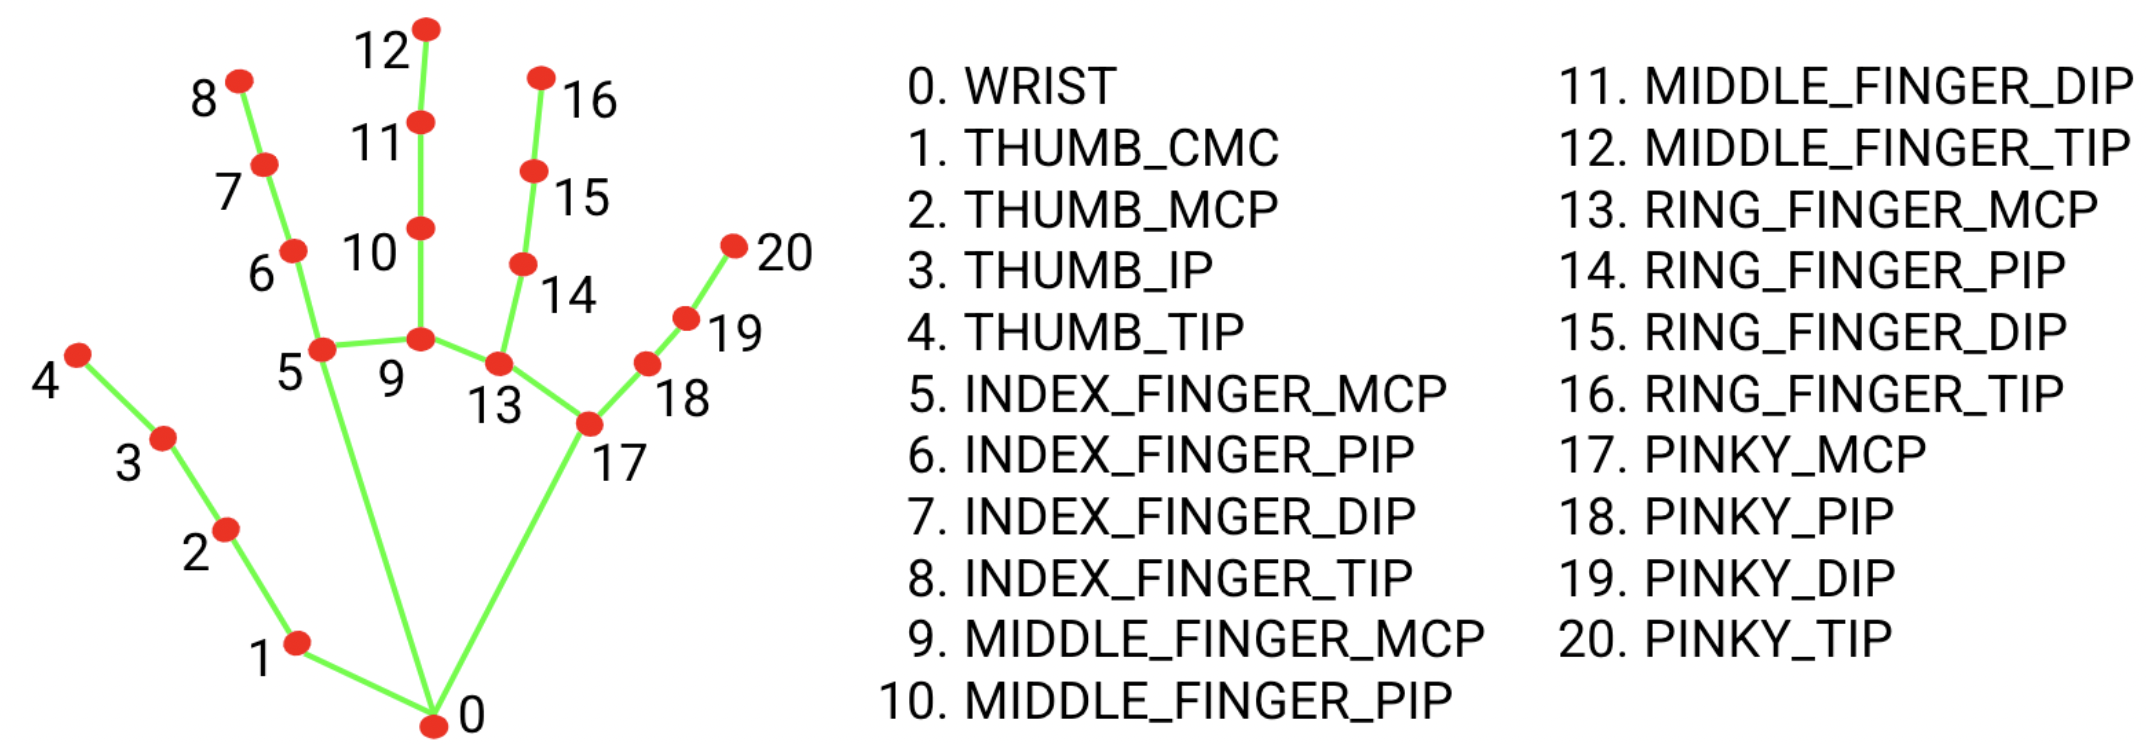
\includegraphics[totalheight=5cm]{hand-landmarks.png}
    \caption{ییییس}
    \label{fig:verticalcell}
\end{figure}


\section{اهمیت ژست دست}
وقتی مردم صحبت می کنند، ژست می گیرند. ژست جزء اساسی زبان است که اطلاعات معنادار و منحصر به فردی را انتقال می‌دهد. ژست‌ها به گوینده کمک می‌کنند تا اهداف خود را بهتر منعکس کند. 
آن‌‌ها نقش های بسیاری را در ارتباط، یادگیری و درک هم برای افرادی که آنها را مشاهده می کنند و هم برای کسانی که آنها را ایجاد می کنند، ایفا می کنند.
وقتی مردم صحبت می کنند، دستان خود را حرکت می دهند. به حرکات خود به خودی دست که در ریتم گفتار ایجاد می شوند، حرکات هم گفتاری \LTRfootnote{co-speech gestures}
نامیده می شوند و مردم از همه فرهنگ ها و پیشینه های زبانی شناخته شده ژست می گیرند و برای ارتباط از حرکات هم گفتاری برای رساندن بهتر مفهوم خود کمک می‌گیرند.
در واقع، نوزادان قبل از اینکه اولین کلمات خود را بیان کنند، از انواع ژست‌ها استفاده می‌کنند. دست‌های ما به ما کمک می‌کنند صحبت کنیم، فکر کنیم، و به خاطر بسپاریم، گاهی دانش
منحصر به فردی را که هنوز نمی‌توان به زبان آورد، آشکار می‌کنند. به طوری که می‌توان گفت ژست‌ها اغلب به عنوان زبان گفتاری ثانویه در نظر گرفته می شود.\cite{clough2020role}
ژست‌ها به‌ویژه زمانی مؤثر هستند که مزیتی نسبت به کلمات داشته باشند. \cite{kang2016hands}
توانایی درک شکل و حرکت دست‌ها می‌تواند یک جزء حیاتی در بهبود تجربه کاربر \LTRfootnote{user experience} 
در حوزه‌ها و پلتفرم‌های مختلف فناوری باشد. درک مفهوم ژست دست در زمان واقعی برای افراد به طور طبیعی وجود دارد، یک کار بینایی 
کامپیوتری کاملاً چالش برانگیز است، زیرا دست ها اغلب خود یا یکدیگر را مسدود می کنند مانند انسداد انگشت، کف دست و لرزش دست و فاقد الگوهای کنتراست بالا هستند.\cite{zhang2020mediapipe}

\section{کنترل پهپاد}
اکثر پهپادهای تجاری موجود در بازار یا دارای کنترلرهای طراحی شده ویژه هستند، یا دارای فرستنده سیگنال اختصاصی و برنامه‌های نرم‌افزاری هستند که روی دستگاه‌های دستی کاربران 
مانند تلفن‌های همراه یا تبلت‌ها اجرا می‌شوند. در هر دو مورد، کنترل‌کننده فرمان‌هایی را با اطلاعات دقیق از طریق کانال‌های بی‌سیم مانند 
وای‌فای یا بلوتوث ارسال می‌کند. اخیراً محصولات تجاری وجود داشته است که حرکات دست را به عنوان یک مکانیسم کنترل قابل اجرا معرفی می کنند. برای گرفتن ژست ها، دو رویکرد وجود دارد.
\begin{itemize}
    \item	استفاده از دستکش های طراحی شده ویژه: کنترل کننده بر روی دستکشی که توسط کاربران استفاده می شود نصب می شود و در زمان واقعی انحراف، گام و چرخش دست را شناسایی می کند 
    تا به حرکات مربوطه برای پهپاد را شناسایی و ارسال کند. محصولات عبارتند از \lr{Kd Interactive Aura Drone} و \lr{MenKind Motion Control Drone}
    \item 	استفاده از بینایی کامپیوتر از طریق دوربین: این دستگاه‌ها از دوربین نصب شده روی پهپاد استفاده می‌کنند تا بتوانند در لحظه تشخیص دهند که دست کاربر کجاست
    و در چه حالتی قرار دارد تا پهپاد را کنترل کند. محصولات عبارتند از \lr{DJI Spark Drone} 
\end{itemize}





